% board-warping-lenses/bw_si_fisheye.tex — generated by board-warping-lenses/tools/board_warping_lenses.py; do not edit.
% One 3-D panel: the estimated height field of set bw_si_fisheye as a surface over the page (1000 x 1000 mm; x to the right, y up the page,
% z the height in mm, towards the camera), spline camera, refine product 3ca456c8d4327789. 5 x 5 mesh points; every patch has
% the colour of its band (0.5 mm). Orthographic view (azimuth 20, elevation 38 degrees) with the heights 50 times as large as
% lengths on the page: the axis' height is chosen so that PGFPlots' filling of width x height is exactly that projection. The box is
% -3 ... +3 mm in every panel. Its width is \rcpanelwidth, of which 10 pt at the left hold the tick labels.
\providecommand{\rcfigdir}{src/fig}%
\providecommand{\rcpanelwidth}{\linewidth}%
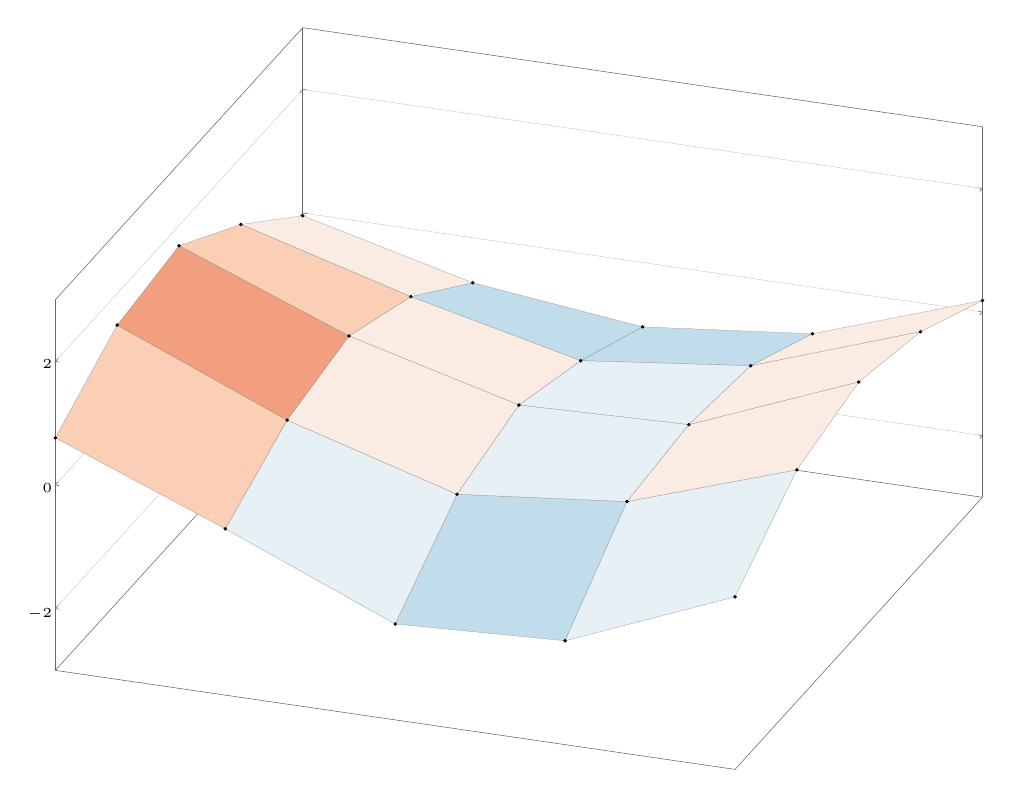
\begin{tikzpicture}[baseline=(current axis.center)]
\pgfmathsetlengthmacro{\rcwarpw}{\rcpanelwidth-10pt}%
\begin{axis}[
  scale only axis, width=\rcwarpw, height=0.80010*\rcwarpw, view={20}{38},
  xmin=0, xmax=1000.0, ymin=0, ymax=1000.0, zmin=-3, zmax=3, clip=false,
  xtick=\empty, ytick=\empty, ztick={-2,0,2}, zticklabel style={font=\tiny, inner sep=1pt},
  tick style={line width=0.2pt, black!60}, major tick length=1.5pt, zmajorgrids, grid style={line width=0.15pt, black!22},
  axis line style={line width=0.2pt, black!60},
  colormap={warp}{rgb255=(17,71,128) rgb255=(42,113,178) rgb255=(74,151,197) rgb255=(139,193,220) rgb255=(193,221,236) rgb255=(231,240,244) rgb255=(250,235,227) rgb255=(251,206,182) rgb255=(241,159,126) rgb255=(216,102,81) rgb255=(187,42,52) rgb255=(134,10,36)}, colormap access=piecewise const, point meta min=-3, point meta max=3]
\addplot3[surf, shader=faceted, faceted color=black!45, line width=0.08pt, mesh/rows=5, z buffer=sort, point meta=z] coordinates {
(0.0,0.0,0.765) (250.0,0.0,-0.308) (500.0,0.0,-1.447) (750.0,0.0,-1.318) (1000.0,0.0,-0.206)
(0.0,250.0,1.489) (250.0,250.0,0.351) (500.0,250.0,-0.448) (750.0,250.0,-0.166) (1000.0,250.0,0.749)
(0.0,500.0,1.671) (250.0,500.0,0.612) (500.0,500.0,-0.105) (750.0,500.0,-0.022) (1000.0,500.0,1.069)
(0.0,750.0,0.916) (250.0,750.0,0.148) (500.0,750.0,-0.488) (750.0,750.0,-0.170) (1000.0,750.0,0.782)
(0.0,1000.0,-0.045) (250.0,1000.0,-0.729) (500.0,1000.0,-1.042) (750.0,1000.0,-0.753) (1000.0,1000.0,0.186)
};
\addplot3[only marks, mark=*, mark size=0.4pt, black] coordinates {(0.0,1000.0,-0.045) (250.0,1000.0,-0.729) (500.0,1000.0,-1.042) (750.0,1000.0,-0.753) (1000.0,1000.0,0.186) (0.0,750.0,0.916) (250.0,750.0,0.148) (500.0,750.0,-0.488) (750.0,750.0,-0.170) (1000.0,750.0,0.782) (0.0,500.0,1.671) (250.0,500.0,0.612) (500.0,500.0,-0.105) (750.0,500.0,-0.022) (1000.0,500.0,1.069) (0.0,250.0,1.489) (250.0,250.0,0.351) (500.0,250.0,-0.448) (750.0,250.0,-0.166) (1000.0,250.0,0.749) (0.0,0.0,0.765) (250.0,0.0,-0.308) (500.0,0.0,-1.447) (750.0,0.0,-1.318) (1000.0,0.0,-0.206)};
\end{axis}
\pgfresetboundingbox\path ([xshift=-10pt]current axis.south west) rectangle (current axis.north east);   % the box is the axis and the strip of the tick labels
\end{tikzpicture}%
